\subsection{\texttt{ci-tools}}

\defverbatim\tmpverb{
    \scriptsize
    \begin{verbatim}
$ git log --format='%ad %an %s' --date=format-local:%Y-%m-%d | tail -3
2018-01-31 Steve Kuznetsov Initial implementation of the ci-operator code
2018-01-31 Steve Kuznetsov Initialize vendor directory with Glide
2018-01-31 Steve Kuznetsov Initialize .gitignore
    \end{verbatim} %$
}

\begin{frame}
    \autotitle
    \footnotesize
    \only<1>{\url{https://github.com/openshift/ci-tools/graphs/contributors}}
    \vfill
    \centering
    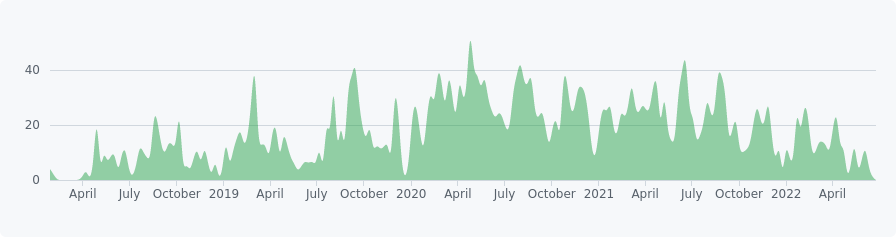
\includegraphics[width=\linewidth]{img/contributors.png}
    \only<1>{\tmpverb}
    \vfill
    \includegraphics<2>[scale=.4]{img/contributors_bbguimaraes.png}
    \note<1>{
        Here is the contributor graph for \texttt{ci-tools}, going back to 2018
        --- the small mount at the beginning is 31 Jan.  You can see the
        "initial implementation of […] \texttt{ci-operator}" in the \texttt{git}
        log.

        None of the original authors remains in the team (in fact, only one
        remains in the company), but the code lives on.
    }
    \note<2>{
        I am the chief code deleter \texttt{=)} (these numbers make little sense
        since we include the \texttt{vendor} directory in the repository)

        I was involved but not directly participating in the beginning, back
        then we were part of the "CI/CD" team and I worked on both sides of the
        slash.  The first thing I remember working on was the implementation of
        the \texttt{--target} argument, although my version is not the one in
        the repository (development was chaotic at the time).
    }
\end{frame}

\begin{frame}[fragile]
    \autotitle
    \tiny
    \begin{verbatim}
$ git log --format='%ad %an %s' --date=format-local:%Y-%m-%d --graph 78af6eb7c
* 2019-06-13 Bruno Barcarol Guimarães Merge Makefiles
*   2019-06-13 Bruno Barcarol Guimarães Merge ci-operator-prowgen
|\
…
| * 2018-08-23 Steve Kuznetsov Add an OWNERS file
| * 2018-08-23 Steve Kuznetsov Reorganize code, add Makefile
| * 2018-08-23 Steve Kuznetsov Copy content from openshift/release
*   2019-06-13 Bruno Barcarol Guimarães Merge ci-operator
|\
…
| * 2018-04-06 Clayton Coleman Add .gitignore for binary
| * 2018-02-09 Steve Kuznetsov Refactor StepLink to be functional
| * 2018-02-08 Steve Kuznetsov Add the release tagging step
| * 2018-02-02 Steve Kuznetsov Add a dry-run mode to the entrypoint
| * 2018-01-31 Steve Kuznetsov Initial implementation of the ci-operator code
| * 2018-01-31 Steve Kuznetsov Initialize vendor directory with Glide
| * 2018-01-31 Steve Kuznetsov Initialize .gitignore
* 2019-06-13 Bruno Barcarol Guimarães Initial commit
    \end{verbatim} %$
    \note{
        If you've ever looked at the repository's history, you might have seen
        it is a bit strange.  There are commits named "merge
        \texttt{Makefile}s", "merge \texttt{ci-operator-prowgen}", and "merge
        \texttt{ci-operator}", followed by forks in the history (n.b.: not
        branches) with their own histories and initial commits, and finally an
        "initial commit" a year and a half \emph{later}.
    }
\end{frame}

\begin{frame}
    \autotitle
    \small \let\small\footnotesize
    \begin{itemize}
        \item \url{https://github.com/openshift/ci-tools.git}
        \begin{itemize}
            \item \url{https://github.com/openshift/ci-operator.git}
            \item \url{https://github.com/openshift/ci-operator-prowgen.git}
            \item \ldots
        \end{itemize}
    \end{itemize}
    \note{
        This is because it started its life as multiple separate repositories
        that were later joined into what is now \texttt{ci-tools}.  Its
        precursors can still be found in Github and are still occasionally of
        historical significance (pull requests and issues are still there).
    }
\end{frame}

\begin{frame}[fragile]
    \autotitle
    \tiny
    \begin{verbatim}
$ git log --format=%ad --date=format-local:'%a %u' --author 'Bruno Barcarol Guimarães' \
    | sort | uniq -c | sort -nk 3,3 \
    | gnuplot …


  140 +--------------------------------------------------------------------+
      |           +          +           +         126          +          |
      |                                          *******                   |
  120 |-+                               112      *     *                 +-|
      |                               ******     *     *                   |
      |                     101       *    *     *     *                   |
  100 |-+                 *******     *    *     *     *                 +-|
      |                   *     *     *    *     *     *                   |
      |                   *     *     *    *     *     *       76          |
   80 |-+        71       *     *     *    *     *     *     ******      +-|
      |        ******     *     *     *    *     *     *     *    *        |
   60 |-+      *    *     *     *     *    *     *     *     *    *      +-|
      |        *    *     *     *     *    *     *     *     *    *        |
      |        *    *     *     *     *    *     *     *     *    *        |
   40 |-+      *    *     *     *     *    *     *     *     *    *      +-|
      |        *    *     *     *     *    *     *     *     *    *        |
      |        *    *     *     *     *    *     *     *     *    *        |
   20 |-+      *    *     *     *     *    *     *     *     *    *      +-|
      |        *    *     *     *     *    *     *     *     *    *        |
      |        *  + *     *  +  *     *  + *     *  +  *     *  + *        |
    0 +--------------------------------------------------------------------+
                 Mon        Tue         Wed        Thu         Fri
    \end{verbatim} %$
    \note{
        Other things you find when excavating through \texttt{git} logs: back
        then, development was \emph{very} chaotic, and Saturday/Sunday pushes
        were not uncommon.
    }
\end{frame}

\begin{frame}[fragile]
    \autotitle
    \tiny
    \begin{verbatim}
$ git log --format=%ad --date=format-local:'%a %u' --author 'Clayton Coleman' \
    | sort | uniq -c | sort -nk 3,3 \
    | gnuplot …


  60 +---------------------------------------------------------------------+
     |        +        +      53        +        +        +       +        |
     |                       *****                                         |
  50 |-+                     *   *                                       +-|
     |                       *   *              44                         |
     |                       *   *             *****                       |
     |                       *   *             *   *                       |
  40 |-+     35              *   *     37      *   *                     +-|
     |      *****     33     *   *    *****    *   *     34                |
     |      *   *   ******   *   *    *   *    *   *   ******              |
  30 |-+    *   *   *    *   *   *    *   *    *   *   *    *            +-|
     |      *   *   *    *   *   *    *   *    *   *   *    *              |
     |      *   *   *    *   *   *    *   *    *   *   *    *              |
  20 |-+    *   *   *    *   *   *    *   *    *   *   *    *    18      +-|
     |      *   *   *    *   *   *    *   *    *   *   *    *   *****      |
     |      *   *   *    *   *   *    *   *    *   *   *    *   *   *      |
     |      *   *   *    *   *   *    *   *    *   *   *    *   *   *      |
  10 |-+    *   *   *    *   *   *    *   *    *   *   *    *   *   *    +-|
     |      *   *   *    *   *   *    *   *    *   *   *    *   *   *      |
     |      * + *   *  + *   * + *    * + *    * + *   *  + *   * + *      |
   0 +---------------------------------------------------------------------+
             Mon      Tue     Wed      Thu      Fri      Sat     Sun
    \end{verbatim} %$
\end{frame}
